% To add this template to the main.tex file, just add the command "\include{titlePageSLU} after "\begin{docuemnt}" in the main.tex file


% In this segment, enter the desired data to be shown at the title page
\newcommand{\thesisAuthor}{Mahnoor Fatima}
\newcommand{\thesisTitle}{Electronic Experiments for STEM Outreach}
\newcommand{\thesisSubTitle}{little bit more descriptive}
\newcommand{\thesisTitleTranslated}{Translated Headline}
\newcommand{\thesisDegree}{Master thesis project}
\newcommand{\university}{Swedish University of Argicultural Science, SLU}
\newcommand{\credits}{30 hp}
\newcommand{\faculty}{Faculty of blablabalba}
\newcommand{\thesisPlaceDate}{Place of puplication, Year}
\newcommand{\company}{Company name}

%------------------------------------------------------------------------------
\begin{titlepage}
\thispagestyle{empty}

% Use this line of code if both SLU loggo and company/other institution loggo is desired. The positions are possible to change with the \hspace and \vspace syntax.


% Adds background picture. Delete code if no background picture is wanted.
\begin{comment}
\begin{tikzpicture}[overlay, remember picture]
\node[anchor=south west] 
     at (current page.south west)
      {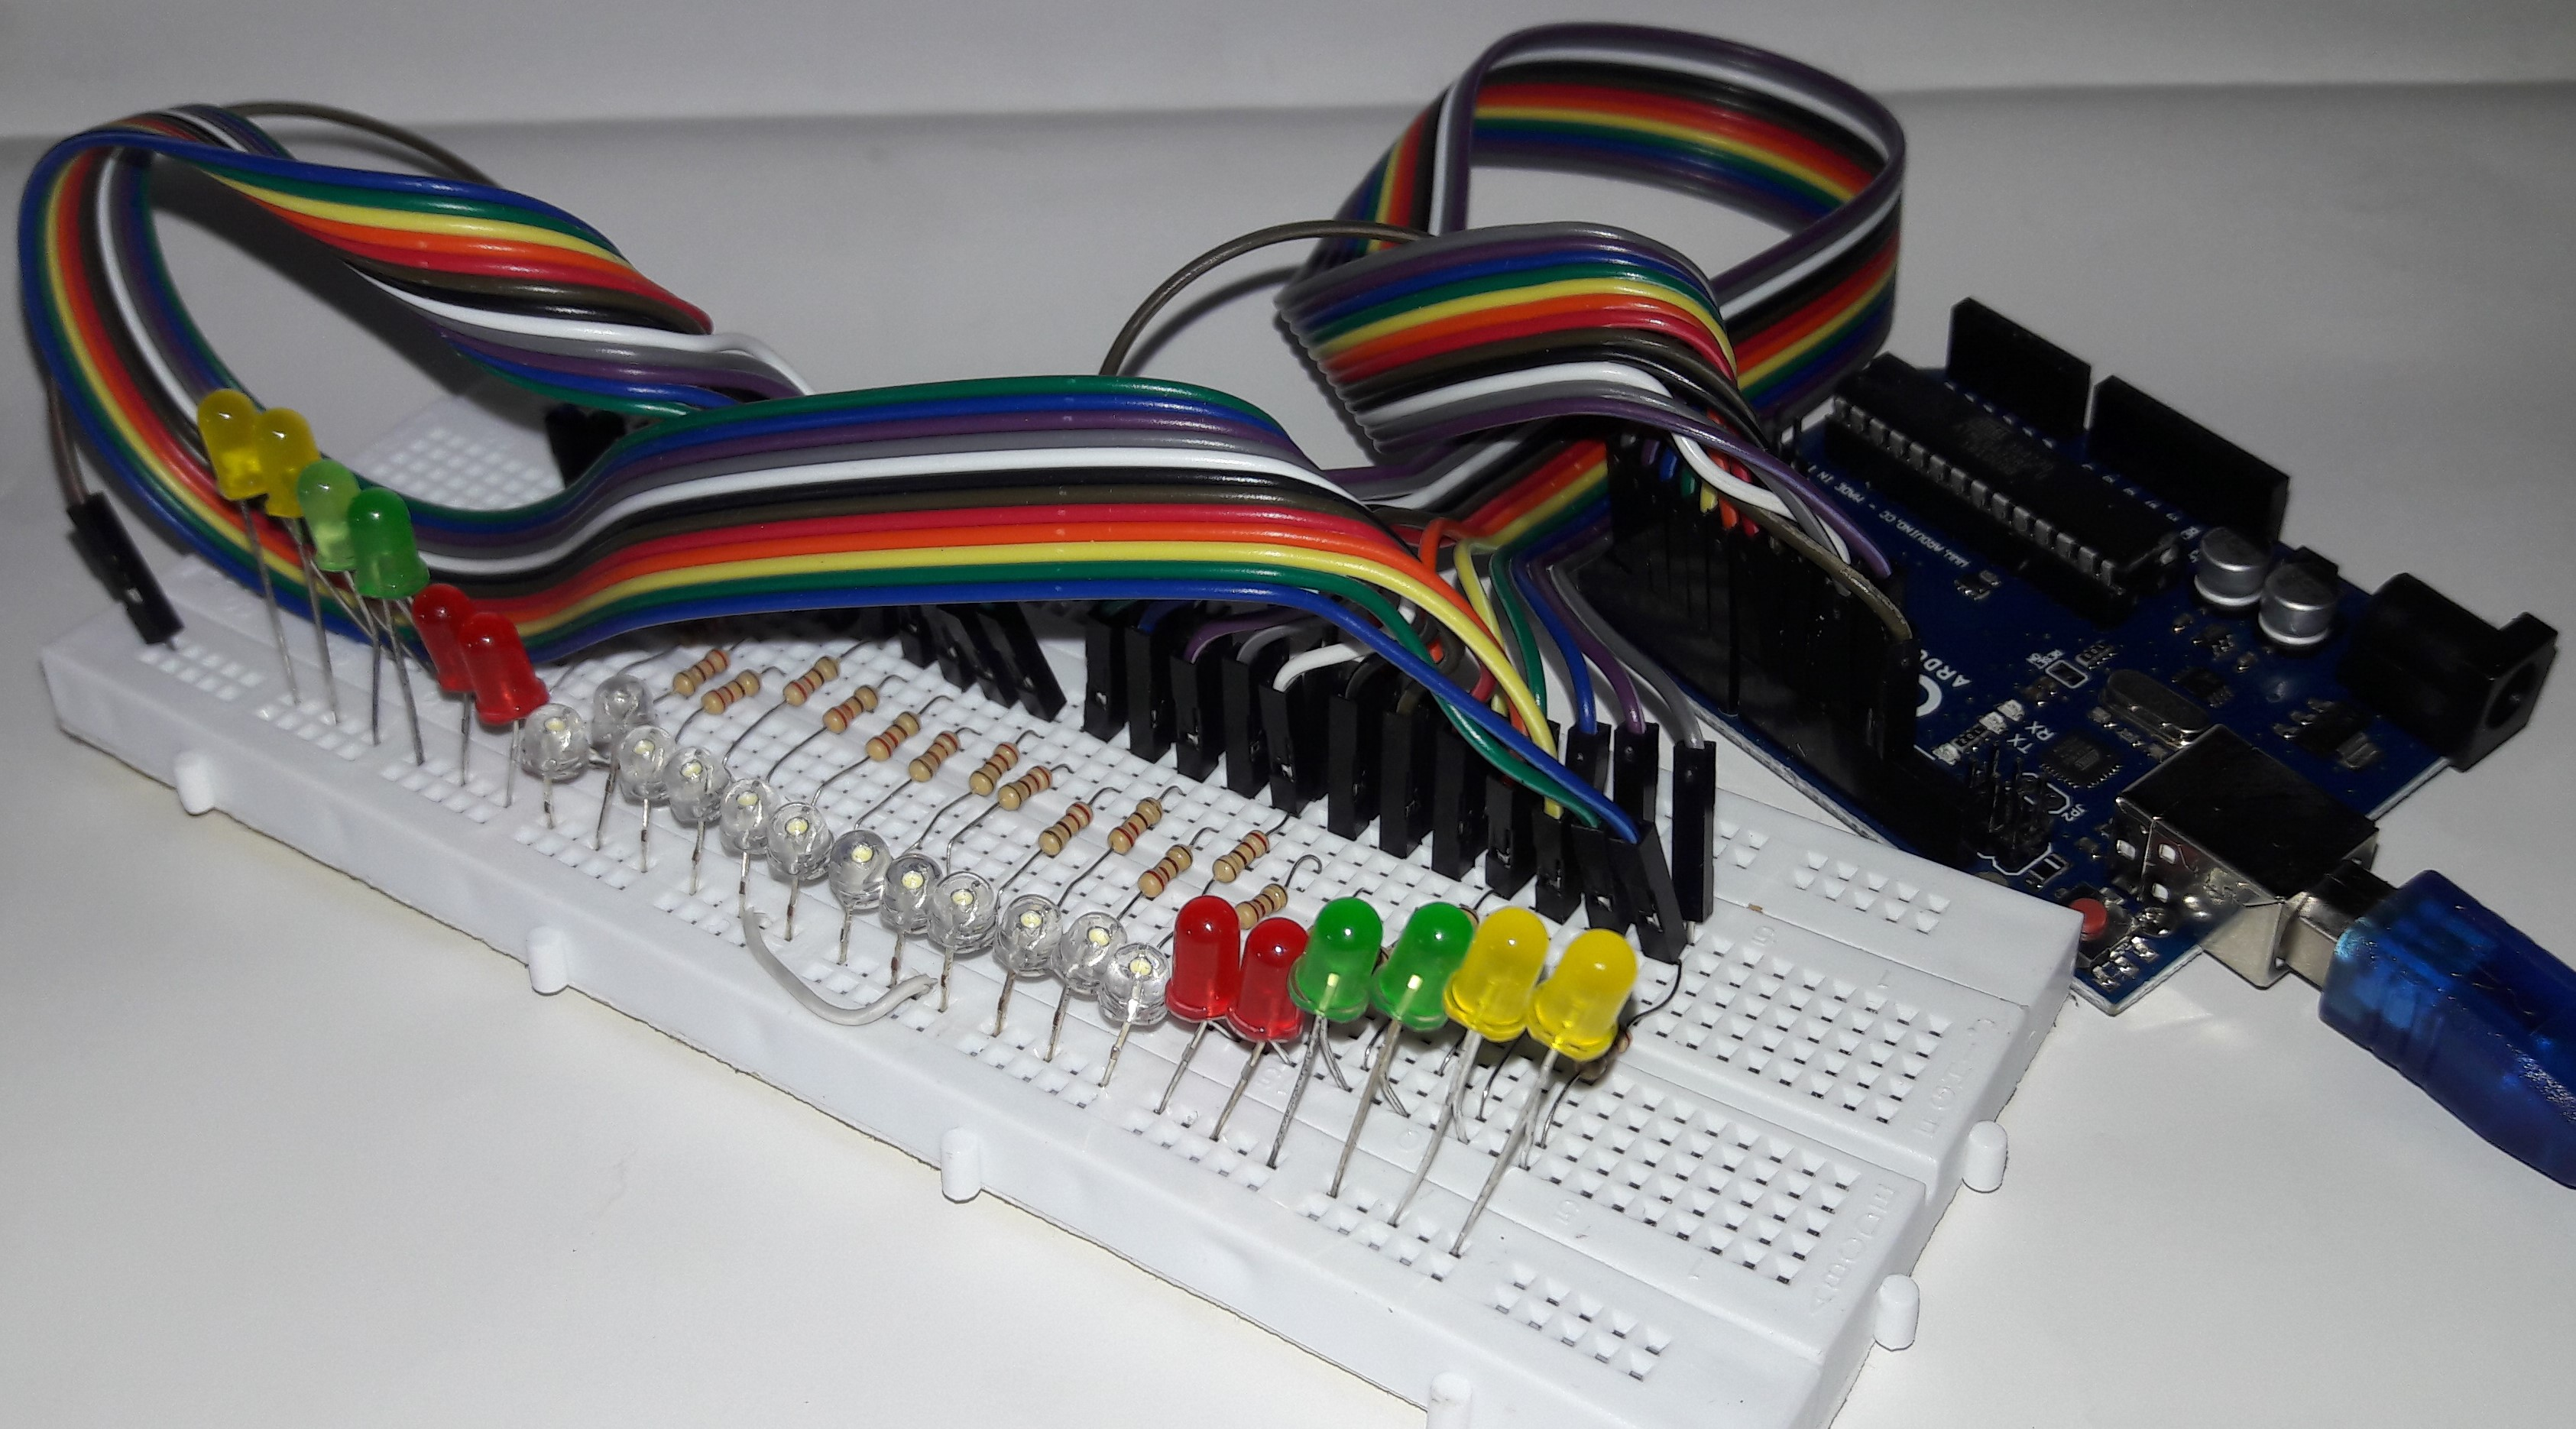
\includegraphics[width=\linewidth]{Figures/recreational_exp/experiment_pics/led pattern.jpg}};
\end{tikzpicture}
\end{comment}

\hspace{2cm}
\centering
\vspace{3cm}
\par
\noindent
\Huge
\rule[0.3cm]{\linewidth}{2pt}
\textbf{Electronic Experiments \\for \\STEM Outreach}\\
\vspace{0.2cm}
\rule[0.3cm]{\linewidth}{2pt}
\Large

\vspace{8cm}

\noindent
\LARGE
\thesisAuthor\\
Ali Khalid\\
\end{titlepage}
